\subsection{Methods and Analysis}

% \todo capital income -- imputed, but not used as an outcome

% \todo we will include health conditions at age 30 in covariates of health dynamics

% \todo health as a child -- are we going to ignore this?

% \todo summarize disease conditions at age 30? -- important point: one female in control group has cancer at age 30

\subsubsection{Overview}
\label{section:FAM_models}

\noindent We develop models to estimate the determinants of transitions between health outcomes, labor market outcomes, educational attainment, and family formation, for individuals aged 25 and older.
Additionally, we estimate transition probabilities by gender, race and ethnicity, and educational attainment as a function of individual characteristics (see below).
Each transition model includes a subset of variables and relevant interactions from the following list: age, gender, race and ethnicity, education, parents' education, self-reported body mass index (BMI), smoking history, physical activity, binge drinking, lagged health conditions, asthma diagnosis before age 30, number of biological children, past earnings and work status, partnership status (single, cohabiting, married, separated/divorced, or widowed), disability status, and health insurance status.
We consider three racial and ethnic groups (black non-Hispanic, white non-Hispanic, and Hispanic), and four educational groups (less than high school degree; high school graduate, including some college or associate's degree; college; and more than college).

\noindent The health transition models estimate the probability that a person transitions between health states, e.g. obesity or heart disease, as a function of current health status, demographic characteristics (including race, gender, age, and education), and risk factors (including weight, smoking status, physical activity, asthma, and number of births if female for BMI transitions), enabling us to age the cohorts. This mechanism to model health transitions accounts for the fact that certain health conditions increase the likelihood of comorbidities.
We estimate a transition model for each of the following health conditions: heart disease, blood pressure, stroke, lung disease, diabetes, and cancer. Each disease model includes gender, race and ethnicity, and educational group as covariates.
We select conditions that are prevalent in the U.S. and are characterized by significant disparities in outcomes across education, race and ethnicity, and income.
The reason for this is that the incidence and progression of these conditions can potentially be reduced by preventive services, education policies, and modifications in health behaviors.
These chronic conditions are treated as absorbing states, i.e., once the individual transitions into a chronic condition, the condition persists until death.

\noindent Additionally, we allow individuals to transition in and out of risk factors, such as smoking, binge drinking, and BMI. These transitions are estimated as a function of demographics, past health, and risk factors.
In the estimation, changes in risk behaviors alter future health outcomes and risk factors (e.g., smoking cessation may impact changes in BMI, and continuing smoking may affect incidence of lung disease). We also transition mental health, approximated by the Kessler mental distress scale, which is one of the predictors of the medical costs models.

%describe models of ADLs IADLs estimation

\noindent Because the PSID sample covers a broad age range, it is smaller than the HRS sample at older ages where mortality becomes more likely. Also, the PSID does not follow respondents into nursing homes.
Therefore, the FAM mortality model is estimated using a pooled PSID and HRS sample.
The mortality model includes these covariates: age, gender, race and ethnicity, education, disease conditions, ADL count, binge drinking and current smoking status.
Similarly, a partner mortality model is estimated from the pooled PSID and HRS data for transitions into widowhood.
The covariates in the partner mortality model are age, gender, race and ethnicity, and education.
These covariates are characteristics of the respondents, not the partners who are facing mortality (FAM does not simulate the characteristics of partners).

\noindent Since the PSID does not follow respondents into nursing homes, the model for nursing home residency is estimated using only HRS data. It is based on these covariates: age, gender, race and ethnicity, education, disease conditions, ADL and IADL counts, and widowhood.

\noindent The marriage transition model estimates transitions between partnership status (we distinguish between single, cohabiting, and married).
The model is a function of demographics, past employment status, earnings, mother's education and number of children.
There are also childbearing models that estimate new births for each gender.
Childbearing is modeled as an ordered Probit model that is a function of past health and birth history, demographics, education, past work status, and past partnership status.

\noindent The employment status model estimates the probability that a person transitions into different employment states (unemployed, out of the labor force, working part-time, or working full-time). This transition is a function of demographics, marital or partnership status, education, health status and behaviors, past earnings and benefits claiming.

% \todo health insurance category -- once it is implemented

% \todo SSI/DI/SS benefits claiming -- once it is implemented

\noindent The combination of transition models allows us to address the aspects of the life-cycle that are most relevant for the proposed analysis. To complete the analysis, there are also models to estimate QALYs, medical expenditure, and Social Security participation.

\noindent We compute a QALY model based on the EQ-5D instrument, a widely-used, health-related
quality-of-life (HRQoL) measure. %\footnote{Section \ref{sec:model_development_qalys_hrqol} gives some background on HRQoL measures.}
The scoring system for EQ-5D was first developed using a U.K. sample.\footnote{\citet{Dolan_1997_Modeling_MC}.} Later, a scoring system based on
a U.S. sample was generated.\footnote{\citet{Shaw_etal_2005_EQ5D_MC}.} The PSID does not ask the appropriate questions for computing EQ-5D, but the MEPS does.

% review this:
\noindent We forecast EQ-5D scores from the MEPS onto the PSID data using common measures between the MEPS and PSID.

We map EQ-5D scores from the MEPS onto PSID data using common variables between the MEPS and PSID. We then run a linear regression of EQ-5D on PSID variables that are transitioned in FAM (including ADL counts, IADL counts, and diseases).\footnote{The main variables in this prediction are self-reported health and requiring help with ADLs.} The microsimulation uses this linear regression to compute QALYs.
%
%We use a crosswalk from MEPS to compute EQ-5D scores for PSID respondents.\footnote{Section \ref{sec:model_development_qalys_eq5d}
%describes EQ-5D in MEPS. Details of the crosswalk model development are given
%in \ref{sec:model_development_qalys_crosswalk}.}.
%The FAM has a more limited specification of functional status than what is available in the PSID. In order to predict
%HRQoL for the FAM simulation sample, we needed to build a bridge between the FAM-type functional status and the
%predicted EQ-5D score in the PSID. We use ordinary least squares to model the EQ-5D score predicted as a function of the six chronic conditions and the FAM-specification of functional status,
%%%


\noindent FAM has two versions of each medical cost model. For individuals who are not Medicare-eligible, the cost models are estimated from MEPS data.
Once an individual becomes Medicare-eligible, their costs are estimated from MCBS data. Both sets of models include the following covariates:
age, gender, race and ethnicity, education level, relationship status, disease conditions, and earnings.
The MEPS models also include type of health insurance as a covariate.
Because MCBS follows respondents for more than two years (the time step length in the FAM simulation), the FAM cost models for the Medicare-eligible population include covariates for the stage of each disease.
In the initial stage, a patient has a diagnosis in the current two-year period, but did not have the diagnosis in the previous two-year period.
Then, in the maintenance stage, a patient had a diagnosis in the previous two-year period and survives with the diagnosis in the current two-year period (all disease states are absorbing---it is impossible to transition out of a diagnosis).
Finally, in the terminal stage, a patient has a diagnosis and dies in the current two-year period.
The medical costs models tend to underestimate health care spending reported in the National Healthcare Expenditures Account (NHEA) data, due in part to underreporting of Medical costs in MEPS.

% Pasted from estimation in Technical Appendix:
\subsubsection{Formalizing the FAM: Modeling Transition Probabilities}
\label{section:transition_models}

We start by providing a formalization of how the FAM models health-state transitions. Examples of health states include heart disease, hypertension, and stroke. We then clarify how the formalization of the health-state transitions is adapted when modeling other outcomes. Examples of these other outcomes include smoking, body-mass index, and binge drinking. We drop individual subscripts to avoid notational clutter.

Let $\mathcal{M}$ denote a set of possible health states, some of which can be absorbing. Transition times are ages of measurement. Let $\mathcal{A}:= [ 0, \ldots, \bar{A}]$ index ages, where $\bar{A}$ is the last age that we forecast. We provide more details on $\bar{A}$ below. We define $h_{a,m,m'}$ as the probability of transitioning from state $m$ to state $m'$ at age $a \in \mathcal{A}$, where $m, m' \in \mathcal{M}$.

We denote a state transition from $m$ to $m'$ at age $a$ by $D_{a,m,m'} = 1$. If this transition does not happen,  $D_{a,m,m'} = 0$. We let $\tilde{D}_{a,m}$ be the indicator of occupancy of state $m$ at age $a$. $\tilde{D}_{a,m} = 0$ otherwise. $\tilde{D}_{a,m}$ is a generic entry in the the vector of age-$a$ state occupancy indicators denoted by $\tilde{\bm{D}}_a$. $\tilde{\bm{D}}_0$ denotes the vector of initial state conditions.

We assume that the transition probability from state $m$ to state $m'$ at age $a$, $h_{a,m,m'}$, is generated by the following index threshold-crossing competing risks model
\begin{eqnarray}
I_{a,m,m'} &=& \bm{\mathit{1}} \left( \tilde{\bm{D}}_{0} \geq 0 \right) \bm{\Omega}_{a,m,m'} + \bm{\mathit{1}} \left( \tilde{\bm{D}}_{a-1} \geq 0\right) \bm{\Lambda}_{a,m,m'}  + \bm{W_a} \bm{\beta}_{a,m,m'}  \nonumber \\ 
&+&  \bm{B} \bm{\alpha}_{a,m,m'} + \tau \left( a \right)_{m,m'} + \varepsilon_{a,m,m'}, \label{eq:trans}
\end{eqnarray}
where $D_{a,m,m'} = \bm{\mathit{1}}  \left( I_{a,m,m'} \geq 0 \right)$; $\tau \left( a \right)_{m,m'}$ is a function of age;\footnote{In our empirical analysis, we approximate the coefficients on $\tau \left( a \right)_{m,m'}$ using splines with knots at ages 35, 45, 55, 65, and 75.} and $\varepsilon_{a,m,m'}$ is a time-varying age-$a$ shock, uncorrelated across ages, subjects, and health states. As in the forecasts of Section~\ref{section:cbamethodology} we allow the transitions models to depend on baseline variables, denoted by $\bm{B}$, and on variables that can be affected by treatment, which in this case we denote by $\bm{W}_a$ to reinforce that they are not the same variables that we use in Section~\ref{section:cbamethodology}. The variables in $\bm{W}_a$ contain health outcomes and other economic outcomes that are modeled with adapted versions of Equation~\eqref{eq:trans} (e.g.,\ smoking, labor force participation, childrearing). $ \bm{\Omega}_{a,m,m'},  \bm{\Lambda}_{a,m,m'}, \bm{\beta}_{a,m,m'},  \bm{\alpha}_{a,m,m'}$ are the coefficient vectors associated to the initial state indicators, first-order lagged state indicators, current health and other economic outcomes, and baseline variables. In our empirical analysis, we estimate these vectors for each $a \in \mathcal{A}$ and for each possible state transition from $m$ to $m'$ with $m,m' \in \mathcal{M}$.

Equation~\eqref{eq:trans} is an adaptation of the framework in \citet{Heckman_1981_heterogeneity,Heckman_1981_IncidentalParametersProblem}. We simplify the modeling and computational procedure in a fundamental way: We do not include a model for initial conditions, and instead allow the index $I_{a,m,m'} $ to be a function of the vector of initial conditions, $\tilde{\bm{D}}_{0}$.

The state probabilities in FAM are derived from Equation~\eqref{eq:trans}. When simulating the model to forecast the health outcomes for the ABC/CARE subjects, we use their observed age-30 conditions as initial conditions  $\tilde{\bm{D}}_0$. The simulation proceeds in an analogous fashion to the simulation in Section~\ref{section:cbamethodology}. The vector $\tilde{\bm{D}}_0$ could have been affected by treatment. \citet{Campbell_Conti_etal_2014_EarlyChildhoodInvestments} the wide variety of effects on health outcomes that ABC/CARE had. This motivates the inclusion of health into our analysis.

\noindent The parameter vector $\bm{\theta} := \left[ \left\{ \left\{  \bm{\Omega}_{a,m,m'}, \bm{\Lambda}_{a,m,m'}, \bm{\beta}_{a,m,m'}, \alpha_{a,m,m'}, \tau \left( a \right) _{m,'m}  \right\}_{a \in \mathcal{A}} \right\}_{m \in \mathcal{M}} \right]$ is estimated by maximum likelihood. Given the normality distribution assumption on $\varepsilon_{a,m,m'}$, the joint probability of all time-intervals until failure, right-censoring, or death conditional is the product of normal univariate probabilities. Since these sequences independent across states, the joint probability over all disease-specific sequences is simply the product of those probabilities.

\noindent For a given subject observed from the initial age, $0$, to the last age, $\bar{A}$, the probability of the observed health history is (omitting the conditioning on covariates for notational simplicity). For each individual for parameter vector $\theta$ is
\begin{equation}
\mathsterling = \prod_{m \in \mathcal{M}} \prod_{a \in \mathcal{A}} {h_{a,m,m'}(\theta)}^{[D_{j,m,m'}]} \prod_{a \in \mathcal{A}}{ h_{a,\bar{M}} }, 
\end{equation}
\noindent where $ h_{a,\bar{M}}$ denotes the probability of transitioning to death, and which parameterization we subsume into $\bm{\theta}$. In our empirical analysis, we deterministically set $\bar{A}$ to be $150$. When fitting the model, no individual survives to $a = 100$.

We use modified versions of the model in Equation~\eqref{eq:trans} to model the following additional health outcomes: 

\begin{enumerate}
\item \textbf{Absorbing states.} A state $m \in \mathcal{K} :\subseteq \mathcal{M}$ is absorbing if $\Pr \left( D_{m,m',a} = 1 \right) \forall m \in \mathcal{K}$.
\item \textbf{Binary states.} States that are not absorbing states, such as the event of starting to smoke.
\item \textbf{Ordered threshold models.} States which transitions are modeled based on a version of Equation~\eqref{eq:trans} recognizing that the observed states is a function of unknown thresholds $\varsigma_m$. Similar to binary outcomes, we allow for state-dependence by including the lagged states on the right-hand side.
\item \textbf{Continuous outcomes modeled as linear models.} An example of a continuous outcome is the
transitions in log(BMI). We allow for state-dependence by including the lagged outcome on the right-hand side. We replace latent variables in Equation~\eqref{eq:trans} with realized variables.
\item \textbf{Categorical models, but without an ordering.} For example, an individual can transition
to being unemployed, out of the labor force, or working (either part- or full-time). In cases like this, we utilize
a multinomial Logit model, including the lagged outcome on the right-hand side.
\end{enumerate}

The modification of the likelihood function to include the estimation of the parameters characterizing these outcomes is straightforward. The economic outcomes that we include are labor income, for which we use the forecast in Section~\ref{section:cbamethodology}, and three additional economic outcomes which we list and briefly explain their forecast next:

\begin{enumerate}
\item \textbf{Employment Status.} We aim to simulate whether an individual is unemployed, out of the labor force, working part-time, or working full-time at age $a$. We do these in two steps. First, we forecast whether the individual is unemployed, out of
the labor force, or working for pay using a multinomial Logitmodel. Then, conditional on working for pay, we estimate if the individual is working part- or full-time using a Probit model.
\item \textbf{Family Relationship Status.} We are interested in three relationship statuses: single, cohabiting, and married. In each case, we treat the transition from age $a$ to age $a+1$ as a two-stage process. First, we estimate if the individual will remain in his current status. Second, we estimate which of the two other states the individual will transition to, conditional on leaving his current state.
\item \textbf{Childbearing.} We estimate the number of children born in two-age periods separately for females and males. We model this using an ordered Probit with three categories: no new births, one birth, and two births. Based on the PSID data, we found the exclusion of three or more births in a two-year period to be appropriate.
\end{enumerate}

With Equation~\eqref{eq:trans} and its modified versions in hand, a crucial aspect is important to clarify before: Outcomes \textit{are not mutually exclusive}. For example, a subject can simultaneously have heart disease and a stroke. In fact, having a stroke at age $a-1$ is a determinant for having heart disease at age $a$. But not only having a stroke but also being disabled, smoking, and having health insurance. It is in this sense that our FAM is a model of competing risks. Equation~\eqref{eq:trans} allows that by letting $I_{a,m,m'}$ depend on not only an indicator of state $m$ at age $a-1$ but a vector of health states at age $a-1$ and other health and economic outcomes at age $a$. 

Tables~\ref{table:supertab1} to ~\ref{table:supertab3} list the variables determining each of the states and health and economic outcomes that we consider. For each of these we list: (1) its classification---e.g., state, binary outcome, continuous outcome; (2) initial states allowed to determine it---$\tilde{\bm{D}}_0$ in Equation~\eqref{eq:trans}; (3) lagged health states allowing to determine it---$\tilde{\bm{D}}_{a-1}$ in Equation~\eqref{eq:trans}; (4) other health and economic outcomes allowing to determine it---$\bm{W}_a$ in Equation~\eqref{eq:trans}; (5) background variables allowing to determine it---$\bm{B}$) in Equation~\eqref{eq:trans}. In that way, the reader could know with certainty the type of outcome being model, its classification, as well determinants and their categorization according with Equation~\eqref{eq:trans}. The outcomes that help predicting each other are based on research and advice of clinicians, as explained and justified in \citet{Goldman_etal_2015_Future-Elderly-Model-Report}.

\textbf{Supertabs go here}.

\paragraph{Specification Tests for the First-order Markov Assumption in FAM} \label{section:firstorder}

\noindent The FAM model assumes a vector first-order Markov process for health states. In Equation~\eqref{eq:trans}, $\tilde{D}_{a - \ell}$ only enters into the model when $\ell = 1$. For heart disease, hypertension, and stroke, we contrast Equation~\eqref{eq:trans} with the following extension: 

\begin{eqnarray}
I_{a,m,m'} &=& \bm{\mathit{1}} \left( \tilde{\bm{D}}_{0} \geq 0 \right) \bm{\Omega}_{a,m,m'} + \bm{\mathit{1}} \left( \tilde{\bm{D}}_{a-1} \geq 0\right) \bm{\Lambda}_{a,m,m'}  + \bm{\mathit{1}} \left( \tilde{\bm{D}}_{a-1} \geq 0\right) \tilde{\bm{\Lambda}}_{a,m,m'} \nonumber \\ 
&+&  \bm{W_a} \bm{\beta}_{a,m,m'}  \bm{B} \bm{\alpha}_{a,m,m'} + \tau \left( a \right)_{m,m'} + \varepsilon_{a,m,m'}, \label{eq:trans1}
\end{eqnarray}

We use a likelihood test ratio to test the null hypothesis $H_0: \tilde{\bm{\Lambda}}_{a,m,m'}$ in Equation~\eqref{eq:trans1}. Table~\ref{table:lrtests} show the results from these tests. For the health states considered, we do not reject the null hypothesis.

\begin{table}[H]
\begin{threeparttable}
\caption{Tests Comparing First-Order and Second Markov Processes for Disease Transition Specifications} \label{table:lrtests}
\centering
\footnotesize
\begin{tabular}{lccc}
\toprule
Statistic & LR Statistic & Degrees of Freedom & $p$-value \\
\midrule \\
Desease & \\
Heart Disease & 2.18 & 2 & 0.71 \\
Hypertension   & 0.05 & 1 & 0.83 \\
Stroke              & 3.94 & 4 & 0.14 \\
\bottomrule
\end{tabular}
\begin{tablenotes}
\footnotesize
\item Note: This table presents likelihood ratios contrasting the models in Equations~\ref{eq:trans} and~\eqref{eq:trans1} by testing the null hypothesis $H_0: \tilde{\bm{\Lambda}}_{a,m,m'}$. The variables included in the right-hand-side of each model are in Tables~\ref{table:supertab1} to~\ref{table:supertab3}. 
\end{tablenotes}
\end{threeparttable}
\end{table}

\noindent An alternative test for a first-order Markov process is the following: (i) use a linear probability model approximation to a first-order Markov process and the variables in Tables~\ref{table:supertab1} to ~\ref{table:supertab3} for each outcome of interest; (ii) calculate the correlation of the residuals with higher order lagged variables. Tables~\ref{table:1storderresidsheart} to \ref{table:1storderresidstroke} show these correlations. The results of these tests very strongly support a first-order Markov assumption.

\noindent To illustrate how to read these tests consider Table~\ref{table:1storderresidsheart}. This table reports simple first-order Pearson correlations with the indicated variable. The row presents the residuals from forecasting heart disease at age $a+1$ using different orders of lags. The estimated correlations are low.

\begin{landscape}
\begin{table}[H]
\begin{threeparttable}
\caption{Tests for Linear Probability Forecasts of Heart Disease at $a+1$} \label{table:1storderresidsheart}
\scriptsize
\centering
\begin{tabular}{lcccccccccc} \toprule
& \multicolumn{10}{c}{Residuals of Forecast of Heart Disease at age $a+1$} \\
Correlations with	&	Predictor Diabetes &	Hypertension &	Diabetes &	Hypertension &	Diabetes	&	Hypertension &	Diabetes & Hypertension & Diabetes & Hypertension \\
                    &	at $a - 2$ &	at $a - 2$		&	at $a - 3$ & at $a - 3$		& at $a - 4$		& at $a - 4$		& at $a - 5$	& at $a - 5$	& at $a - 6$	& at $a - 6$	\\

\midrule \\
&	-0.002	&	-0.006	&	-0.004	& -0.009 &	-0.017	& -0.020	&	-0.015	&	-0.017 &-0.009	&	0.004	\\
\bottomrule
\end{tabular}
\begin{tablenotes}
\footnotesize
\item Note: This table presents the correlation between the residuals from forecasting heart disease at age $a+1$ and the predictors indicated in each column.
\end{tablenotes}
\end{threeparttable}
\end{table}

\begin{table}[H]
\begin{threeparttable}
\caption{Tests for Linear Probability Forecasts of Hypertension at $a+1$} \label{table:1storderresidshyper}
\centering
\scriptsize
\begin{tabular}{lccccc} \toprule
& \multicolumn{5}{c}{Residuals of Forecast of Hypertension at age $a+1$} \\
Correlations with	&	Predictor Diabetes & Diabetes & Diabetes & Diabetes & Diabetes 	\\
                    & at $a - 2$	& at $a - 3$	& at $a - 4$	& at $a - 5$	& at $a - 6$	\\
\midrule
&	0.003	& 0.009	&	0.012	&	0.008	&	0.001	\\
\bottomrule
\end{tabular}
\begin{tablenotes}
\footnotesize
\item Note: This table presents the correlation between the residuals from forecasting hypertension at age $a+1$ and the predictors indicated in each column.
\end{tablenotes}
\end{threeparttable}
\end{table}

\begin{table}[H]
\begin{threeparttable}
\caption{Tests for Linear Probability Forecasts of Stroke at $a+1$} \label{table:1storderresidstroke}
\centering
\footnotesize
\begin{tabular}{l *{8}{c}}
\toprule
& \multicolumn{8}{c}{Residuals of Forecast of Stroke at age $a+1$} \\
Correlations with	&	Predictor Cancer &	Diabetes & Heart Disease &	Hypertension &	Cancer	& Diabetes & Heart Disease & Hypertension  \\
                    &	at $a-2$	&	at $a - 2$ & at $a - 2$	& at $a - 2$	& at $a-3$	& at $a - 3$	& at $a - 3$	& at $a - 3$ \\
\midrule \\
&	0.004 &	0.008	&	0.001	&	0.001	&	-0.002	&	0.017 &	-0.004 &	-0.001	\\
\bottomrule
\end{tabular}
\begin{tablenotes}
\footnotesize
\item Note: This table presents the correlation between the residuals from forecasting stroke at age $a+1$ and the predictors indicated in each column.
\end{tablenotes}
\end{threeparttable}
\end{table}
\end{landscape}

%
%\subsubsection{Inverse Hyperbolic Sine Transformation}
%One problem fitting the wealth distribution is that it has a long right tail and some negative values. We use a
%generalization of the inverse hyperbolic sine transform (IHT) presented in \citet{mackinnon1990transforming}. First denote the variable of
%interest $y$. The hyperbolic sine transform is
%\begin{equation}
%y = \sinh(x) = \frac{\exp(x) - \exp(-x)}{2}
%\label{eqn:sinh_y}
%\end{equation}
%The inverse of the hyperbolic sine transform is
%\[
%x = \sinh^{-1}(y) = h(y) = \log(y + (1+y^2)^{1/2})
%\]
%Consider the inverse transformation. We can generalize such transformation, first allowing for a
%shape parameter $\theta$,
%\begin{equation}
%r(y) = h(\theta y)/\theta
%\label{eqn:generalized_ihs_shape}
%\end{equation}
%Such that we can specify the regression model as
%\begin{equation}
%r(y) = x\beta + \varepsilon, \varepsilon \sim \mathrm{N}(0, \sigma^2)
%\label{eqn:ihs_regression_model}
%\end{equation}
%A further generalization is to introduce a location parameter $\omega$ such that the new
%transformation becomes
%\begin{equation}
%g(y) = \frac{h(\theta(y+\omega)) - h(\theta\omega)}{\theta h'(\theta \omega)}
%\label{eqn:geralized_ihs_loc_scale}
%\end{equation}
%where $h'(a) = (1+a^2)^{-1/2}$.
%
%We specify (\ref{eqn:ihs_regression_model}) in terms of the transformation $g$. The shape parameters
%can be estimated from the concentrated likelihood for $\theta, \omega$. We can then
%retrieve $\beta, \sigma$ by standard OLS.
%
%Upon estimation, we can simulate
%\[
%\tilde{g} = x \hat{\beta} + \sigma \tilde{\eta}
%\]
%where $\eta$ is a standard normal draw. Given this draw, we can retransform using
%(\ref{eqn:geralized_ihs_loc_scale}) and (\ref{eqn:sinh_y})
%\begin{align*}
%&h(\theta(y+\omega)) = \theta h'(\theta\omega)\tilde{g} + h(\theta\omega)\\
%&\tilde{y} = \frac{\sinh\left[\theta h'(\theta\omega)\tilde{g} + h(\theta\omega)\right]-\theta\omega}{\theta}
%\end{align*}

% \todo link to transition_estimates.xls on box -- make link unique to the version of the appendix in make process
%The included estimates table (estimates\_FAM.xml) gives parameter estimates for the transition models.
% Ends estimation from Technical Appendix.



\subsubsection{FAM simulation}
\label{appendix:health-fam-simulation}

\noindent A simulation of the model starts by loading the entering cohort, generated from the ABC/CARE data. Missing values are imputed with the imputation models described in section \ref{section:FAM_ABC_impute}. To this entering cohort, the model applies the transition models for mortality, health, working status, family structure, wealth, and benefit claiming, estimated from PSID, with Monte Carlo decisions to calculate the new states of the population.
%The simulation is performed 5,000 times and the simulated distributions of key outcomes are summarized over repetitions.
The simulated financial outcomes are in 2014 USD.


\noindent To match the biennial structure of the PSID data used to estimate the transition models, the simulation proceeds in two-year increments.\footnote{The end of each two-year step is designed to occur on July 1st to allow for easier matching with population forecasts from Social Security Administration (SSA).}
Once the new states have been determined, the cross-sectional models for medical costs and QALYs are applied.
Computation of medical costs includes the people who died to account for end-of-life costs.
The simulation ends when all simulated ABC/CARE subjects are deceased (in the simulation).\footnote{Less than half of the simulated subjects (48\%) survive to age 80.} \textbf{[JJH: Actually or in the simulation?] [JLG: In simulation.] [JJH: So it is open ended?] [JLG: In principle, yes. But all of our subjects either die or have QALYs equal to zero at most at age 95.]}

\noindent Among the ABC/CARE subjects simulated in FAM, the years of completion of the age-30 interview range from 2003 to 2009.
FAM's two-year time step only allows the simulation of even or odd years.
For this reason, we ran the simulation twice---once for the ABC/CARE subjects entering in odd years and again for the ABC/CARE subjects entering in even years.

\noindent The simulation model takes as inputs assumptions regarding the normal retirement age, future improvements in mortality, and real medical cost growth.
% \DEL: interest rates assumptions apply to wealth -- not simulated
The normal retirement age is assumed to be 67 for all ABC/CARE subjects.
%% Wage growth has been turned off for this project
%\noindent Real wage growth projections are taken from the intermediate cost projections in Table VI.F6 of the 2009 Social Security Trustees Report\footnote{\citet{Trustees_2009_Annual-Report-Old-Age-Survivors}.} and then assumed to be 1.1\% annually in subsequent years.
%These wage-growth assumptions are plotted in Figure \ref{figure:nwi}. In each year of the simulation, the FAM earnings model predicts a subject's earnings in terms of 2009 USD.
%The earnings are then multiplied by the ratio of the current year index value to the 2009 index value in order to account for real wage growth since 2009. We then inflate our results to 2014 USD. \\

\noindent The FAM mortality model represents mortality rates in 2009.
The estimated mortality probabilities are reduced in simulated future years to represent improvements in mortality from sources such as medical innovation that are not included in the model.
There are different adjustment factors for the populations under and over the age of 65.
The mortality reduction factors are taken from the intermediate cost mortality projections in the 2013 Social Security Trustee's Report.

%% Not using NWI growth in this project
%\begin{figure}
%\caption{National Wage Index} \label{figure:nwi}
% \centering
%	 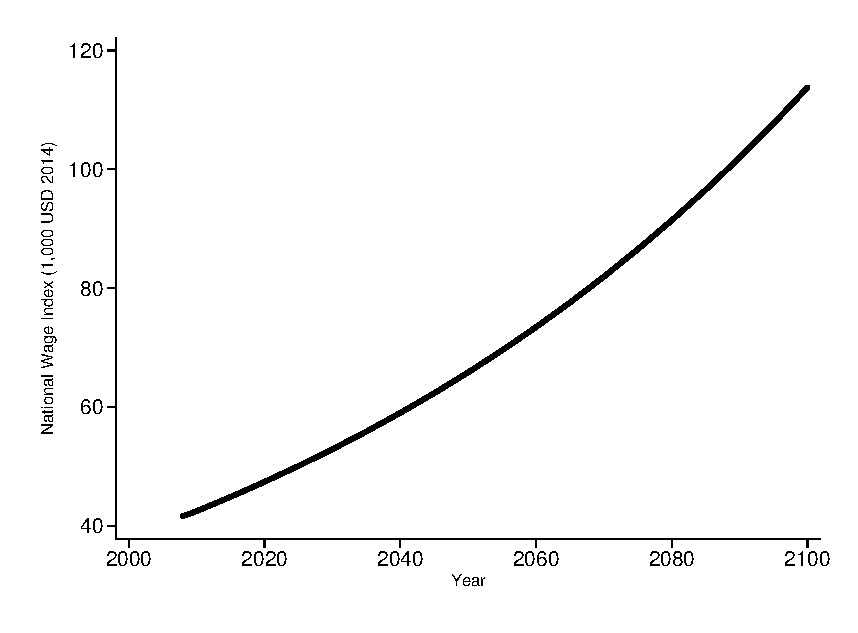
\includegraphics[height=3.5in]{AppOutput/Health/nwi.eps}
%\floatfoot{
%\footnotesize
%\noindent Note: Real wage growth projections are taken from Table VI.F6 in the 2009 Social Security Trustees Report \citep{Trustees_2009_Annual-Report-Old-Age-Survivors}. In years after the Trustees report projections, real wage growth is assumed to be 1.1\% annually.
%}
%\end{figure}

\noindent Medical cost growth assumptions are derived from several underlying assumptions about growth in GDP and the labor force.
The real medical cost growth factor in each year is calculated by first finding the minimum of (i) the year-over-year GDP growth plus year-over-year excess medical cost growth or (ii) the Affordable Care Act cap on year-over-year medical cost growth. In order to obtain the medical cost adjustment factor for the current year of the simulation, FAM takes the cumulative product of the yearly growth factors since 2004 and then divides it by the relative growth in the labor force since 2004.\footnote{The medical cost growth assumptions come from Congressional Budget Office and SSA assumptions.
The year-over-year growth assumptions for medical costs are shown in Figure \ref{figure:medgrowth_yearly}.
The 2010-2019 GDP assumptions are based on CBO's analysis of the President's Budget, March 2009.
GDP assumptions for 2020-2100 are based on the 2008 OASDI Trustee's Report long-term projection of 2.1\% real GDP growth.}


\begin{figure}
\caption{Year-over-Year Excess Real Growth in Medical Costs} \label{figure:medgrowth_yearly}
 \centering
	 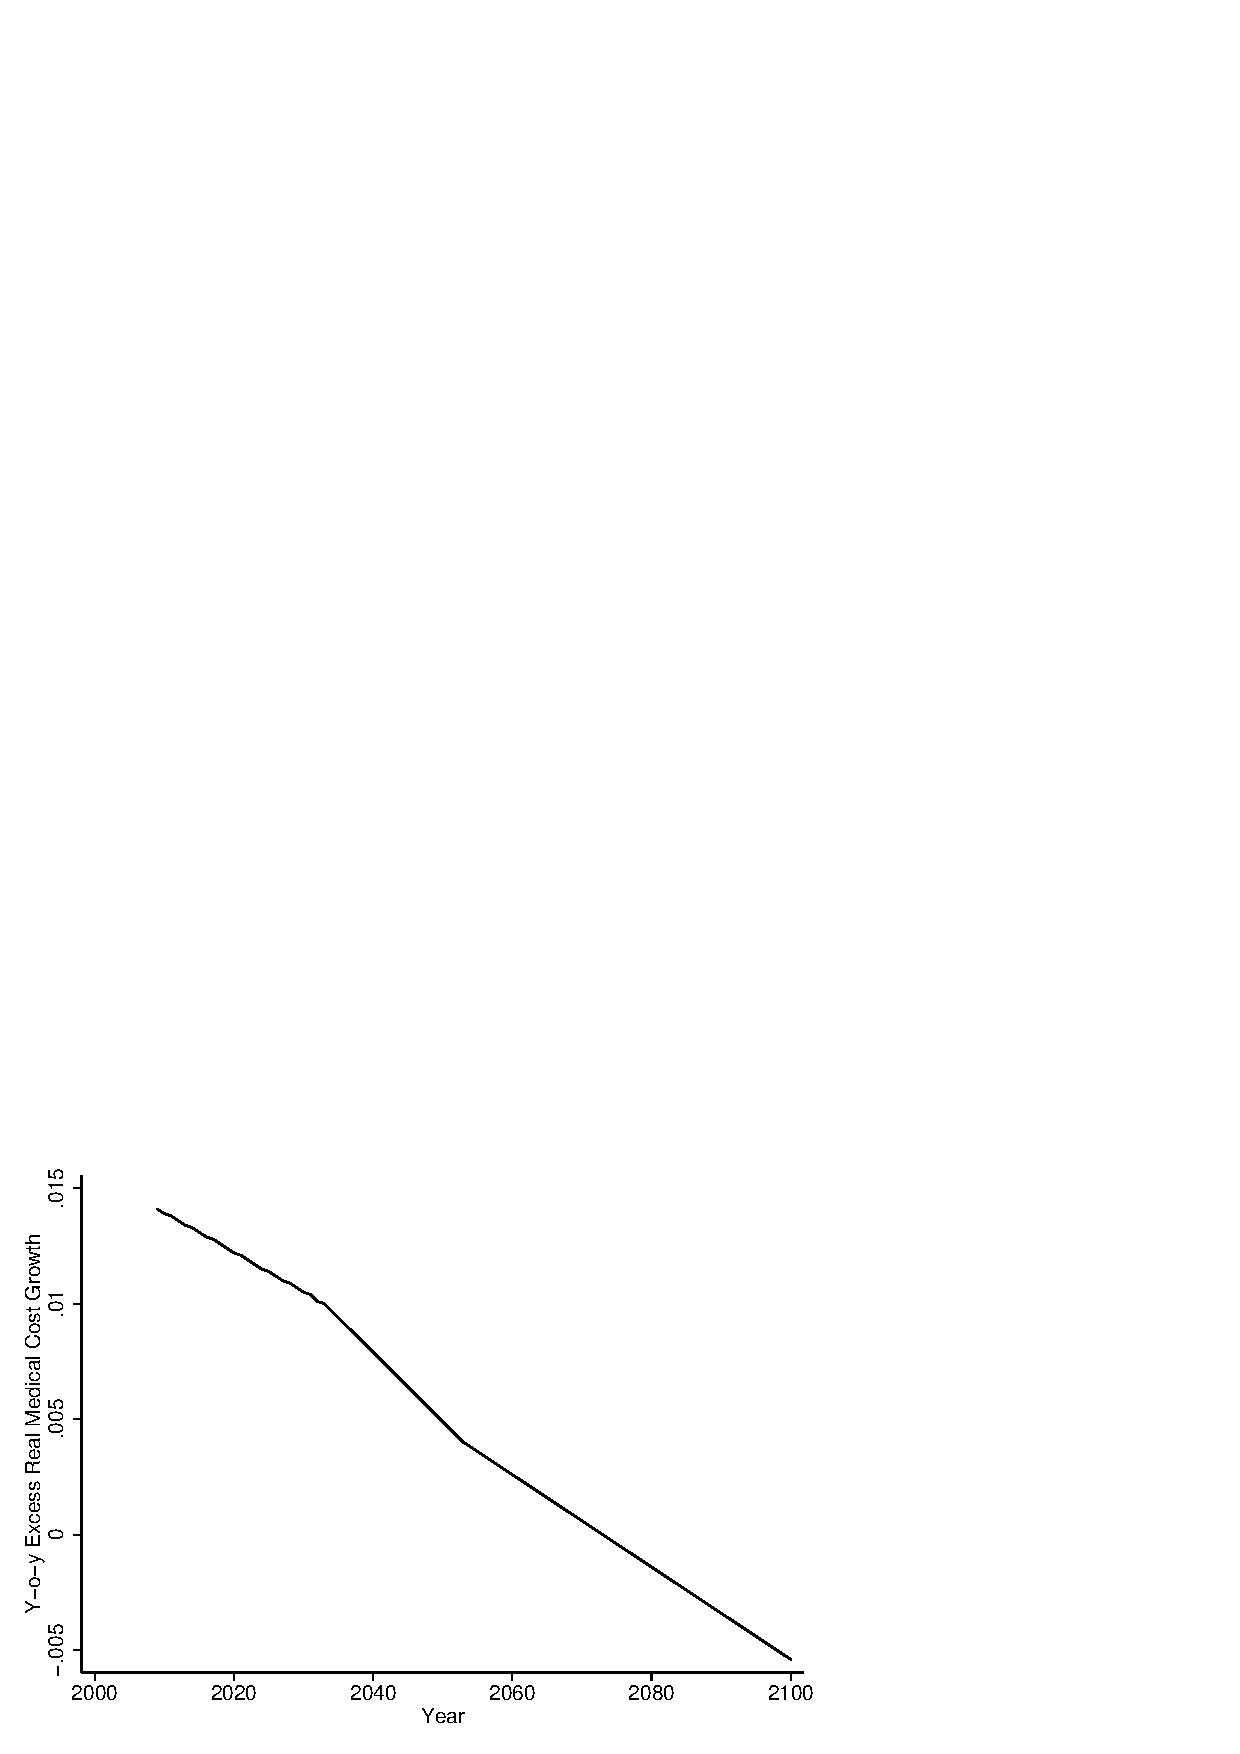
\includegraphics[height=3.5in]{AppOutput/Health/medgrowth_yearly}
\floatfoot{
\footnotesize
\noindent Sources: Congressional Budget Office, Social Security Administration.\\
\noindent Note: The year-over-year excess real medical cost growth over GDP is used to model medical cost growth in FAM.
}
\end{figure}

\begin{comment}
\subsubsection{Bootstrap Sampling Strategy}

\noindent The data sets used for estimating models in FAM are resampled in order to get estimates of sampling error in simulated outcomes. PSID, HRS, MEPS, and MCBS all have complex survey designs that incorporate stratification and clustering. In each of these data sets, the exact sampling strata and clusters are not publicly available, but approximations are included for the purpose of variance estimation. The bootstrap methods in FAM were developed to implement the sampling strategy of \citet{McCarthy-Snowden_1985_Bootstrap}: randomly select $n_h-1$ sampling units with replacement from stratum $h$, where $n_h$ is the number of sampling units in stratum $h$.

\noindent PSID started with an initial sample of families in 1968. Each generation of children from those families became sample members as they formed their own households. The sample members present in the 1999--2013 PSID waves are used to estimate FAM models. The PSID data used for estimation also includes a sample targeting immigrants that entered in 1997. We randomly select one cluster from each variance estimation stratum in the 1968 and 1997 cohorts, with replacement. Any family (original sample members or their descendants) belonging to that cluster are eligible to be included in the estimation for that bootstrap sample.

\noindent The HRS is resampled at the household level. From each variance estimation stratum, $n_h-1$ households are randomly selected with replacement, where $n_h$ is the number of households in the stratum. Observations for each household member are eligible to be included in the estimation for that bootstrap sample.

\noindent In MCBS, $n_h-1$ individuals are resampled with replacement from each variance estimation stratum, where $n_h$ is the number of individual beneficiaries in the stratum.

\noindent MEPS is resampled by dwelling unit. Each MEPS bootstrap sample randomly selects $n_h-1$ dwelling units with replacement from each variance estimation stratum, where $n_h$ is the number of dwelling units in the stratum. All members of the dwelling unit are eligible to be in the estimation sample.
\end{comment}

\subsubsection{Medical Costs Before Age 30 Interview}
\label{appendix:health-costs-before-age30}

\noindent Data on utilization of medical services is sparse before the age 30 interview. There are questions about utilization in the age 12, 15, and 21 interviews along with records of births for female subjects. We combined this with information about demographics, family structure, and parents' utilization of public services to estimate medical costs at each age from 8 to 32. Models were estimated separately for males and females. All imputation and cost models are estimated using MEPS data.

\noindent Medical costs for ages 8 to 11 were estimated in three stages using age 12 interview data. First, we impute whether or not a subject spent a week in the hospital for those subjects who are missing this information in their age 12 interview. The imputation model forecasts utilization based on race and whether or not the subject was ever diagnosed with asthma between ages 8--11. Next we separate the ABC/CARE subjects into the group that spent a week in the hospital in this age range and the group that did not. For the group that did not spend any time in the hospital, we forecast medical costs as a two stage model. The first stage predicts whether there were any medical costs at all. Then, the second stage forecasts the amount of medical costs for those subjects who were predicted to have some costs. We assume the group that spent time in the hospital had some medical costs, so we skip the first stage and go directly to predicting the amount. The cost models use race, asthma diagnosis, whether or not the father was absent from the home, family use of food stamps, and number of siblings as predictors.

\noindent Medical costs for ages 12 to 14 follow a strategy similar to the age 8--11 costs. First, we impute whether or not a subject had any hospitalization for those subjects who do not report this in their age 15 interview. Imputations are based on race and presence or absence of an asthma diagnosis between ages 12--14. Again, we separated the ABC/CARE subjects into a group that had a hospitalization between age 8--11 and a group that did not. A two-stage model was used to forecast medical costs for those with no hospitalization. Medical costs for the group that had a hospitalization were estimated directly from a single-stage model. These cost models use race, asthma diagnosis, whether the mother, father, or both parents were absent from the home, family use of food stamps, and number of siblings.

\noindent To estimate medical costs for ages 15 to 20, we first impute whether or not the subject spent time in the hospital for those who are missing this information in the age 21 interview. The imputation model was based on race, asthma diagnosis between ages 15--20, and, for females, the birth of any children. The age 21 interview asks about the number of days spent in the hospital. However, it does not record the ages at which these hospital stays occurred. Considering the difficulty of assigning the hospital days to specific ages in the absence of other information, we decided to use only the indicator of whether or not there were any days spent in the hospital. Next, we separated subjects into a group that spent some time in the hospital between ages 15--20 and those who did not. As before, we used the direct model to forecast costs for those who had been to the hospital and used a two-stage model for those who had not. The cost models forecast costs based on race, asthma diagnosis, any births (female model only), use of food stamps, whether or not the subject was working age, work status, living at college, and living with parents, and marital status.

\noindent Unlike the interviews at younger ages, the age 30 interview does not ask about utilization of medical services. To estimate costs for ages 21--31, we skipped the utilization imputation step and moved directly to cost models. We used two-stage cost models. The first stage predicts whether or not there were any costs based on race, asthma diagnosis between ages 21-31, education, use of food stamps, any births (female model only), whether or not the subject was working age, living at college, living with parents, and marital status.

\noindent Table~\ref{table:pre30} summarizes individual and family characteristics used to forecast medical expenditure models for each age.

\begin{table}[H]
\begin{threeparttable}
\caption{Health Expenditure Models by Age Group, before Age 30}\label{table:pre30}
\begin{tabular}{lcccc} \toprule
Explanatory variable & \multicolumn{4}{c}{Age Group} \\
& 8-11 & 12-14 & 15-20 & 21-30 \\
\midrule
Race/ethnicity & \checkmark & \checkmark & \checkmark & \checkmark \\
Education        & $\times$ & $\times$ & $\times$ & \checkmark \\
Asthma Diagnoses & \checkmark & \checkmark & \checkmark & \checkmark \\
Hospital stays & if $\geq$ 1 week & any stay & any stay & $\times$ \\
Births & $\times$ & $\times$ & \checkmark & \checkmark \\
Mother present & $\times$ & \checkmark & $\times$ & $\times$ \\
Father present & \checkmark & \checkmark & $\times$ & $\times$ \\
Number of siblings & \checkmark & \checkmark & $\times$ & $\times$ \\
Foodstamps & \checkmark & \checkmark & \checkmark & \checkmark \\
Living arrangements & $\times$ & $\times$ & \checkmark & \checkmark \\
Working, if working age & $\times$ & $\times$ & \checkmark & \checkmark \\
\bottomrule
\end{tabular}
\begin{tablenotes}
\footnotesize
\item Note: This table summarizes the explanatory variables included in the models we use to forecast medical expenditure for each age group. Possible living arrangements are: living with parents, away at college, married, or other.\\
\end{tablenotes}
\end{threeparttable}
\end{table}
